\documentclass[11pt,a4paper]{article}
\usepackage[margin=2.5cm]{geometry}
\usepackage[utf8]{inputenc}
\usepackage[T1]{fontenc}
\usepackage{hyperref}
\renewcommand{\familydefault}{\sfdefault}
\usepackage{helvet}
\pagestyle{empty}
%\usepackage[kerning=true]{microtype}
\usepackage{parskip}
\usepackage{sansmath}
\usepackage[font={small, bf}]{caption}
\usepackage[font={small}]{subcaption}
\usepackage{graphicx}
\usepackage{multicol}
\setlength{\abovecaptionskip}{0pt}
\setlength{\floatsep}{10pt}
\setlength{\textfloatsep}{0pt}
\setlength{\intextsep}{0pt}
\setlength{\belowcaptionskip}{0pt}
\setlength{\parindent}{0ex}
\setlength{\parskip}{0pt}
% Feel free to use additional packages for glosses, figures, whatnot.

% The next bit is for reserving sufficient space for authors,
% affiliations, and e-mail address.  No need to change for initial
% anonymous version.  For the final version, replace the
% \toggletrue{anonymous} with \togglefalse{anonymous} to de-anonymize.
\usepackage{etoolbox}
\newtoggle{anonymous}
\togglefalse{anonymous}
\usepackage{ulem}
\renewcommand{\title}[1]{\textbf{#1}\\}
\newcommand{\authors}[1]{\iftoggle{anonymous}{\phantom{#1}}{#1}\\}
\newcommand{\email}[1]{\iftoggle{anonymous}{\phantom{#1}}{#1}}

\begin{document}

% First page:

% Insert title, authors, affiliations, and e-mail address in the next three lines:
\noindent\title{SOME TITLE}
\authors{Veronica Boyce (vboyce@stanford.edu), Ben Prystawski, Alvin Tan, Michael C. Frank (Stanford University)} 
\newline

%TODO

\textbf{Background:} Word predictability (often measured as surprisal) is a predictor of language processing times, but how rapidly do comprehenders adapt to changing contexts that may license globally uncommon expressions? Does the use of a strange expression become unsurprising with repeated exposure (based on very local context), or does it stay surprising based on overall unexpectedness? 

We use transcripts from iterated reference games as a way to create this globally weird, locally predictable structure. In TODO CITE PNAS paper, groups of people played an iterated reference game where a speaker described a target image so that listeners could pick out that target image from a set of 12 images. Over repeated trials, all images were described 6 times. Descriptions from later rounds were often shorter and often used ideosyncratic nicknames distilled from successful earlier descriptions. 

Methods: For the present experiment, we selected 10 games with above average accuracy, and above average reduction to in-group nicknames, to test how well outsiders could understand the shorthand descriptions and examine their reading time profile. We recruited XX participants who each read trial transcripts and guessed the intended target. Participants first read the transcript by uncovering it word by word in a modified self-paced reading paradigm, and then selected a target image (Figure 1). In the \textbf{yoked} condition, a participant saw all the trials from one game in the order they occurred (72 trials, 6 descriptions of each of 12 targets). In the \textbf{shuffled} condition, a participant seen all the trials from one game in a randomized order. 

Results: Participants had an average target selection accuracy of YY\% (ZZ in the yoked condition, and QQ in shuffled). Accuracy was blah higher and blah whatever (Table 1). 

What is predictive of word-by-word reading times in this task? In addition to the predictors of word length and word frequency, we considered 3 potential measures of the words unexpectedness or information value: 1) surprisal from a vanilla LLM (cite), 2) surprisal from a vision language model, and 3) the K-L divergence between the predicted target distribution at the previous word and including the current from a CLIP model with a MLP output thingy trained on the TODO cite corpora. This last represents how much task-relevant information the word includes based on how much it shifts the model's distribution over possible targets. 
To compare we threw everything into a model and stuff happened. 

\newpage

\begin{center}\textbf{}\end{center}
\begin{minipage}{.4\textwidth}
	\captionof{figure}{Original game}
	{	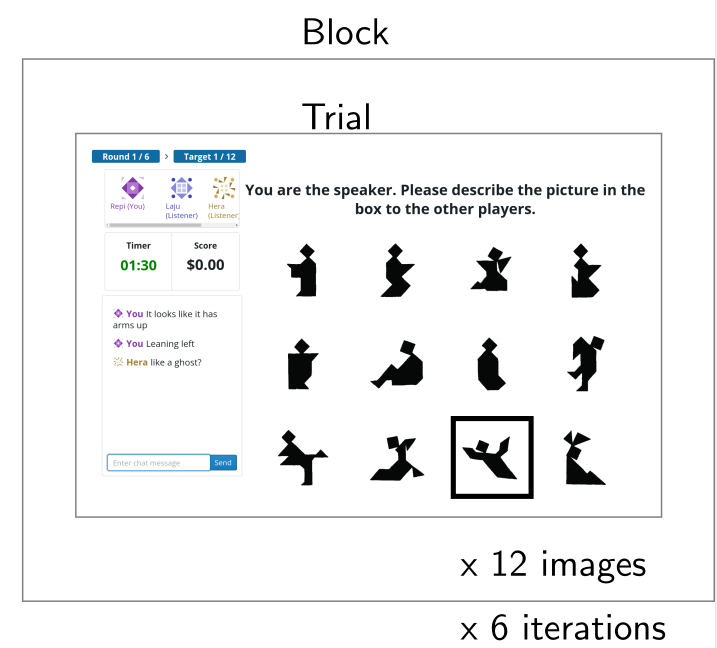
\includegraphics[width=\textwidth]{orig_diagram.png}} 
	
	\begin{small}
	In Boyce et al 2024, participants played a reference game in real time with other participants using a chat box.
	
\end{small}
	
\end{minipage}
~~~
\begin{minipage}{.55\textwidth}
	\captionof{figure}{Current experiment}
{	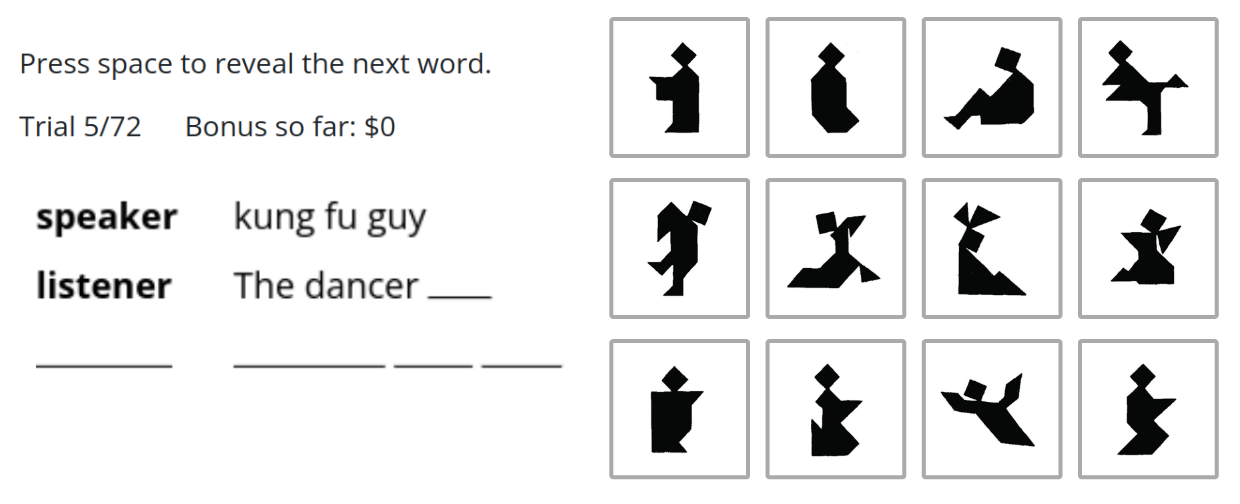
\includegraphics[width=\textwidth]{matcher_diagram.png}} 
\begin{small}
	In the current experiment, we sampled the game transcripts from 10 games from Boyce et al 2024. We recruited new participants to each see the transcripts from one game, either with the trials in the same order (yoked) or a random order (shuffled).  New participants revealed the dialogue from a trial word-by-word and then selected what image they think was being described. 
	
\end{small}	
\end{minipage}


\begin{minipage}{.45\textwidth}
	\captionof{figure}{Accuracy}
	{	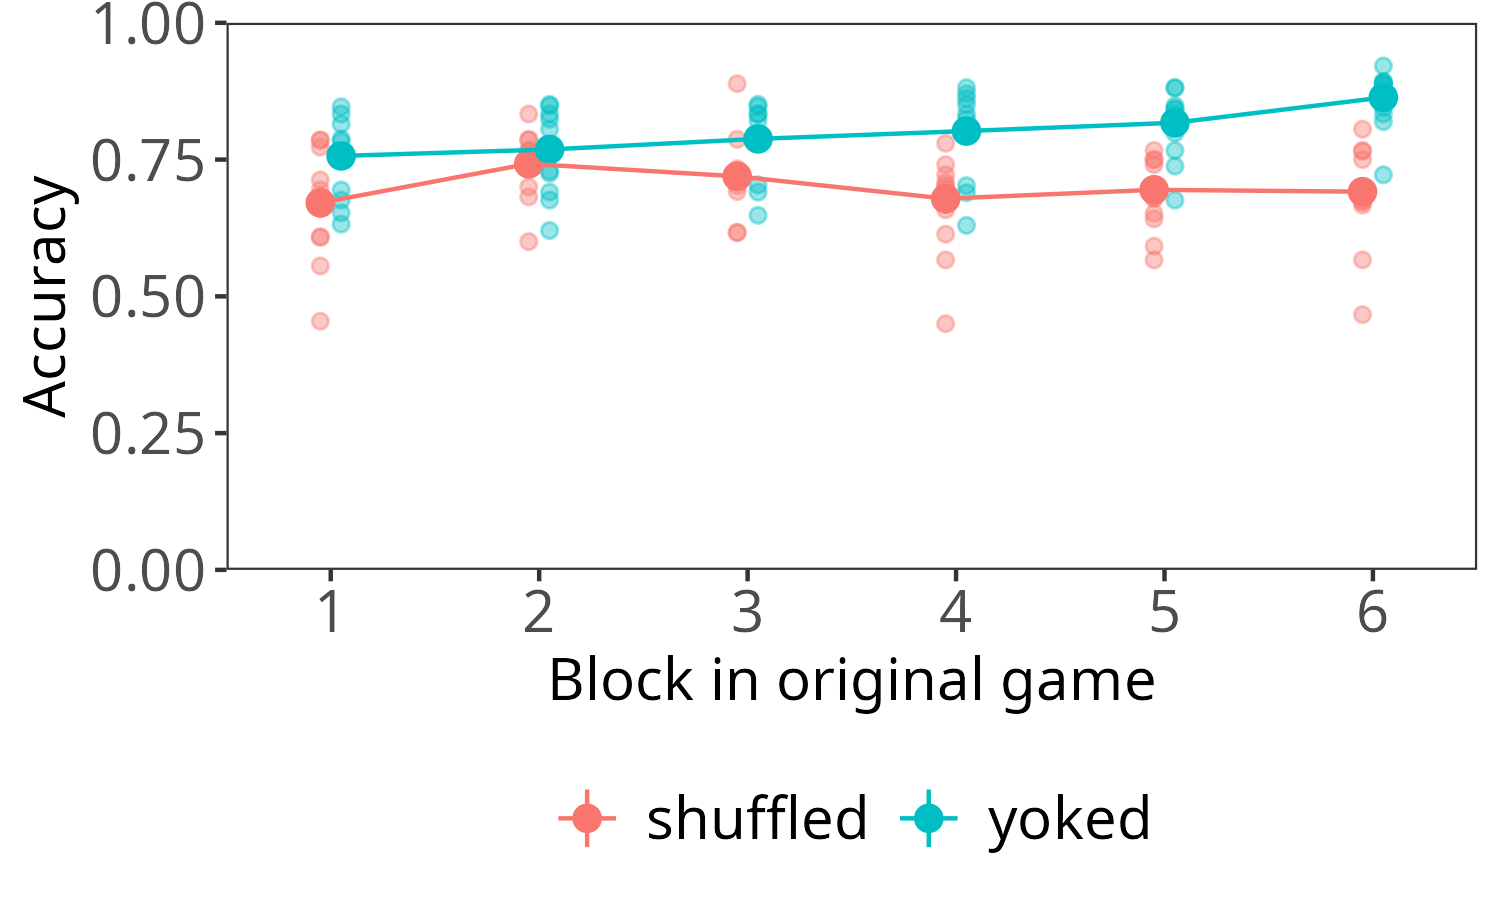
\includegraphics[width=\textwidth]{hsp1.png}} 
	\begin{small}
%
		
	\end{small}
	
\end{minipage}
~~
\begin{minipage}{.5\textwidth}
	\begin{small}
\captionof{table}{Accuracy model}

	\begin{tabular}{|l|l|l|}
		\hline
		Term & Odds Ratio & 95\% CrI \\
		\hline
		Intercept & 1.574 & [.891 -- 2.834] \\
		Original Block & .986 & [.954 -- 1.020] \\ 
		Condition (yoked) & 2.196 & [1.634 -- 3.002] \\
		Block x Condition & .944 & [.889 -- 1.002] \\
		Viewing order & 1.019 & [1.016 -- 1.021] \\
		\hline
	\end{tabular}
	\vspace{2pt}
	
	 Logistic Model: \textit{Accuracy $\sim$  original-block $\times$ condition + order-viewed + (1 | game) + (1 | target) + (1 | participant)  } Coefficients are presented as odds ratios (how much more likely correct responses are).
	 \end{small}
	 	
\end{minipage}

\begin{minipage}{\textwidth}
	\begin{small}
		
		
		
		Model comparison\\
		
		Description of predictors \\
		maybe as diagrams?
		
	\end{small} 
	\medskip
\end{minipage}
\begin{minipage}{\textwidth}
	\vspace{5pt}
	\begin{small} \textbf{References:}%TODO update
Leung, Hawkins, Yurovsky. Cogsci, 2020. $\bullet$ Glucksberg, Krauss, Weisberg. J of Expt Child Psychology, 1966. $\bullet$ Clark \& Wilkes-Gibbs. Cognition, 1986. $\bullet$ Hawkins, Frank, Goodman. Cognitive Science, 2020. $\bullet$ Reimers \& Gurevych. arXiv 2019.
\end{small}
\end{minipage}


\end{document}